\subsection{Conversión de la forma Primal a la Dual}

Para representar la forma dual desde la forma primal se realiza el proceso:
Se puede encontrar la forma dual desde la forma primal realizando varias sustituciones en el lagrangiano, esto es:

\begin{equation}
\begin{split}
\mathcal{L}(x, \pi, s) =& c^T x - \pi^T ( Ax - b) - s^T x \\
=& (c^T - A^T \pi - s) x + \pi^T b  
\end{split}
\end{equation}
Por lo tanto la función Dual se obtiene si:
\begin{equation}
\begin{split}
q(\pi, s) = inf_x \mathcal{L}(x, \pi, s)=& (c^T - A^T \pi - s) x + \pi^T b  
\end{split}
\end{equation}
Entonces se tiene su cota inferior al considerar primer condición $(c^T - A^T \pi - s) = 0$ por lo tanto como resultado se tiene $q(\pi, s) = \pi^T b$.
%

\subsection{Implementación del Algoritmo Simplex}
Este método itera en los puntos básicos factibles que corresponden al polítopo factible.
%
Los puntos básicos factibles corresponden a un vértice del polítopo, por lo tanto de una forma greedy en cada iteración se visita cada vértice adyacente hasta encontrar el punto factible óptimo.
%
En caso de que el problema no esté limitado el procedimiento no terminará, por lo tanto es recomendable asignar un número máximo de iteraciones.
%
En este procedimiento se dividen el espacio que corresponde al problema, donde se considera la base $B$ y sus índices $B_i$ donde cada uno indica la $i$-ésima columna de la matriz de restricciones $A$. 
%

El complemento de $B_i$ es denotado como $N_i$ esto es $N_i = \{1,2,...,b \} \ B_i$.
%
También se particionan los vectores $x$, $s$, $c$ en 

\begin{equation}
\begin{split}
 x_{B_i} = [x_i]_{i \in B_i} & \quad
 x_{N_i} = [x_i]_{i \in N_i} \\
 s_{B_i} = [x_i]_{i \in B_i} & \quad
 s_{N_i} = [x_i]_{i \in N_i} \\
 c_{B_i} = [x_i]_{i \in B_i} & \quad
 c_{N_i} = [x_i]_{i \in N_i}
\end{split}
\end{equation}
Dadas las condicieones se tiene que $Ax = Bx_b + Nx_n = b$.
\\
Las variables primales $x$ para este simplejo iterado es definen de la forma $x_B = B^{-1} b$, $x_N = 0$.
%
Se pueden encontrar los elementos restantes $\pi$ y $s_N$ asignando $S_B=0$ obteniendo $B^T = c_B$ y $N^T \pi + s_N = c_N$.
%
Desde que $B$ es cuadrada y no singular, se obtiene $\pi = B^{-T} c_B$ y se obtiene $s_N = c_N - N^T \pi = c_N - (B^{-1} N)^T c_B$

\begin{algorithm}[!t]
\caption{Simplex}
\label{alg:Simplex}
\begin{scriptsize}
\begin{algorithmic}[1]
\STATE Dados $B_i$, $N_i$, $x_B = B^{-1}b \geq 0, x_N = 0$
\STATE $max_ite =mCn$ (Combinación)
\WHILE{ $max_ite > i$}
\STATE Resolver $B^T \pi = c_B$ para $\pi$.
\STATE Calcular $s_N = c_N - N^T \pi$.
\IF{$s_N \geq 0$}
   \STATE Salir, óptimo encontrado.
\ENDIF
\STATE Seleccionar $q \in N$ con $s_q < 0$ siendo el índice que entrará al conjunto básico.
\STATE Resolver $B t = A_q$ para $t$.
\IF{ $t \leq 0$}
\STATE Salir, el problema no está limitado.
\ENDIF
\STATE Calcular $x_q^+ = min_{i | t_i > 0} (x_B)_i / t_i$, definir el índice $p$ como el índice que corresponde al mínimo valor logrado.
\STATE Actualizar $x_B^+ = x_B - t x_q^+$, $x_N^+ = (0,...,0,x_q^+,0,...,0)$
\STATE Cambiar el conjunto básico de índices $B_i$ agregando a $q$ y en el lugar de $p$\
\STATE $i = i+1$
\ENDWHILE
\end{algorithmic}
\end{scriptsize}
\end{algorithm}

En este método se deben tener en cuenta tres aspectos importantes:
\begin{itemize}
   \item Se puede mantener una factorización LU o QR de la matriz básica $B$ con el fin de resolver $\pi$ y $t$, ya que si $LU = B$, entonces primero se puede resolver $L_{\hat{t}} = A_q$ y después $Ut = \hat{t}$
   \item Se puede implementar algún método más sofisticado para elegir el ínice $q$ como el componente negativo de $s_N$, por lo regular existen varios componentes negativos.
   \item Es importante manejar los pasos degenerados, en donde $x_q^+=0$.
\end{itemize}

El método simplex requiere un punto básico factible y el conjunto básico de indices $B_i \subset \{ 1, 2, ..., n\} $ con $B_i = m$ donde:
\begin{itemize}
   \item La matriz $B$ es no singular y de dimención $m$ $x$ $m$.
   \item $x_B \geq 0$ y $x_N=0$, donde $N_i$ es el complemento de $B_i$.
\end{itemize}

Para encontrar esta información se puede implementar el procedimiento \textit{Phase-I/Phase-II}.
%
Este procedimiento consiste de dos fases, en la fase I se construye un problema auxiliar, este es distinto a la forma estándar, este problema es resuelto por medio del método de simplex.
%
el problema de la fase I es construida de tal forma que es sencillo calcular los  puntos iniciales básicos factibles.
%
Por lo tanto ls solución de la fase I proporciona un conjunto básico factible para la fase II.
%

Posteriormente, en la fase II se resuelve un problema muy similar a la forma estándar, iniciado desde la solución obtenida en la fase I.
%
Por lo tanto la solución del problema se puede obtener de la solución obtenida en la fase II.
%

Particularmente, en la fase I se introducen las variables artificiales $z$, y se re-define la función objetivo como la suma de las variables artificiales.
%
\begin{equation}\label{estandar_artificial}
min \quad \vec{e}^T \vec{z}, \quad sujeto \quad a: \quad A\vec{x} + E \vec{z} = \vec{b}, \quad (\vec{x},\vec{z}) \geq 0
\end{equation}
%
Específicamente, el problema de la fase I es:

donde $z \in \Re$, $e=(1,1,...,1)^T$, y $E$ es la matriz diagonal donde los elemento diagonales son$E_{jj} = +1$ si $b_j \geq 0$, $E_{jj} = -1$ si $b_j < 0$.
%
Se observa que el punto $(x,z)$ es definido por 
\begin{equation}\label{punto_inicial}
x=0, z_j = |b_j|, j=1,2,..,m
\end{equation}

En cualquier punto factible de (\ref{estandar_artificial}), las variables artificiales $z$ representan las cantidades por las cuales se violan las restricciones $Ax = b$ por los componentes de $x$, y la función objetivo esta comprendida simplemente por la suma de estas violaciones, por lo tanto minimizando esta suma se está forzando que $x$ se convierta factible para el problema original (estándar).
%

En general se aplica el método simplex a (\ref{estandar_artificial}) con el punto inicial (\ref{punto_inicial}).
%
Si se obtiene una solución óptima para la cual la función objetivo $e^T z$ es positiva, se concluye que el problema original no es factible.
%
De otra forma el simplex identifica un punto factible para el problema lineal de la segunda fase
\begin{equation} \label{fase2}
min \quad \vec{c}^T \vec{x}, \quad sujeto \quad a: \quad A\vec{x} +  \vec{z} = \vec{b}, \quad \vec{x} \geq 0, \quad 0 \geq z \geq 0
\end{equation}

Este problema es equivalente a la forma estándar, ya que cualquier solucion debería tener $z=0$, es importante mantener las variables artificiales $z$ en la fase II.
%
Además, para evitar iteraciones adicionales, es posible quitar variables artificiales en la fase II.


\begin{algorithm}[!t]
\caption{Algoritmo Simplex de dos fases}
\label{alg:Simplex_fases}
\begin{scriptsize}
\begin{algorithmic}[1]
\STATE Construir la función objetivo que corresponde a la ecuación (\ref{estandar_artificial}).
\STATE \textbf{Fase I}
\STATE Asignar $B_i = z_i$, es decir el conjunto base está conformado por los índices de las variables artificiales indicado en la ecuación \ref{punto_inicial}.
\STATE Obtener $x_B$, $x_N$, $B_i$, $N_i$  el algoritmo \ref{alg:Simplex}, donde $A$ está conformada por $[ A \quad  z]$.
\STATE \textbf{Fase II}
\STATE Construir la función objetivo que corresponde a la ecuación (\ref{fase2}).
\STATE Obtener $x_B$ con  el algoritmo \ref{alg:Simplex}, es importante usar la matriz $A$, los índices del conjunto básico $B_i$, el punto básico factible $x_B$ que se obtuvieron en la fase I.
\end{algorithmic}
\end{scriptsize}
\end{algorithm}

Es posible optimizar este procedimiento por medio de varias estrategias de álgebra lineal, esta implementación se puede considerar como la ingenua ``naive''.
%
Inclusive existen estrategias para seleccionar de forma más eficiente el índice que se ingresará en el conjunto básico de índices.

\subsection{Análisis de rendimiento del método simples}

Para analizar el rendimiento del método Simplex se desarrolló un procedimiento para generar problemas de Programación Lineal (PL).
%
Es importante considerar que la matriz $A$ debe ser de rango completo $rank(A) = m$, para realizar esto existen distintas estrategias:
\begin{itemize}
\item Generar una matriz de forma aleatoria y reducir a su forma triangular con el método de Gauss-Jordan.
\item Generar una matriz de forma aleatoria y obtener la base con el procedimiento de Gram Schmidt, posteriormente agregar las $m$ columnas que sean múltiples de la base.
\item Generar una matriz de forma aleatoria, verificar si es de rango completo en caso de que no lo sea vover a generar otra matriz.
\item Generar un vector $\vec{X}$ de forma aleatoria, construir una matriz de la forma $A = \vec{x}^T \vec{x}$, agregar columnas con factores múltiples a la matriz $A$.
\end{itemize}

Existen otros factores que pueden influir en este proceso, como es el caso en que la matriz está conformada por una gran cantidad de ceros que dependiendo del método para resolver el sistema de ecuaciones ( para $t$ y $\pi$) puede ser más rápido.
%
Además también es importante observar el rango de los número aleatorios, ya que si el rango es elevado se pueden tener problemas de precisión.
%

Para relajar los problemas de precisión se consideran números enteros de forma aleatoria.

Los experimentos de rendimiento consisten en dos grupos:

\begin{itemize}
\item Generar aleatoriamente en su forma estándar para $n=200*i$ con $i \in \{1,2,..,50 \}$ y $m = n/2$.
\item Generar aletoriamente en su forma estándar para $n=2000$ y $m=200*i$ con $i \in \{1,2,...,10\}$
\end{itemize}

El procedimiento para generar la matriz de forma aleatoria corresponde a la última opción de la mencionadas anteriormente donde se genera un vector con números aleatorios y posteriormente se multiplican.
%
El experimento se ejecutó en el cluster ``El insurgente'', una observación interesante es que la configuración de python automáticamente realiza la paralelización en los productos vectoriales, la forma en que se paraleliza esta parte es con memoria compartida.
%
La maquina central donde se realizaron las pruebas consta de 24 procesadores ( físicos 12 con hiperthreading ), la memoria RAM disponible es de 126 Gigabytes.
%
La versión de python es 2.7.12+.
%
El número máximo de iteraciones asignado fue asignado como $min(mCn ,1000000)$ ya que si el número de bases posibles asignadas es a lo más $mCn$, es decir el número de formas de elegir $m$ elementos como base de $n$ índices posibles, y aunque existe un número finito de iteraciones en esta configuración el número de combinaciones pueden aumentar de forma exponencial.


Se puede observar en la figura \ref{img:Media} el comportamiento incremental del tiempo conforme aumenta el número de variables y restricciones, en teoría el límite superior en este caso es $O(n^3)$ ya que no se realiza el cálculo de la inversa $x_B = B^{-1} b$ y por lo tanto no son necesarios demasiados recursos del sistema.
%
Aun que popularmente existen variantes del método Simplex como es el tradicional tableau \cite{bland1977new}, donde de forma continua se realizan operaciones entre filas y columna considerado como una variante del método de Gauss.
%
La implementación que se presenta en este trabajo está basado en el libro de Jorge Nocedal, y puede ser requerir más operaciones ya que se resuelven dos sistemas de ecuaciones, la primera para calcular los valores $\pi$ del lagrangiano y la segunda para el cálculo de la ``Dirección'' $t$.
%
No obstante es importante notar que se puede implementar alguna factorización ($LU$, $QR$ entre otros) teniendo un menor coste computacional, siendo al final equivalente al procedimiento Tableau, y en algunos casos (sistemas ralas o sparse) más eficiente. 
%
Como ya se mencionó el vector basico inicial $x_B$ es generado en la fase I, y para esta primer fase el punto factible ya está definido.
%


\begin{figure*}[h]
\center
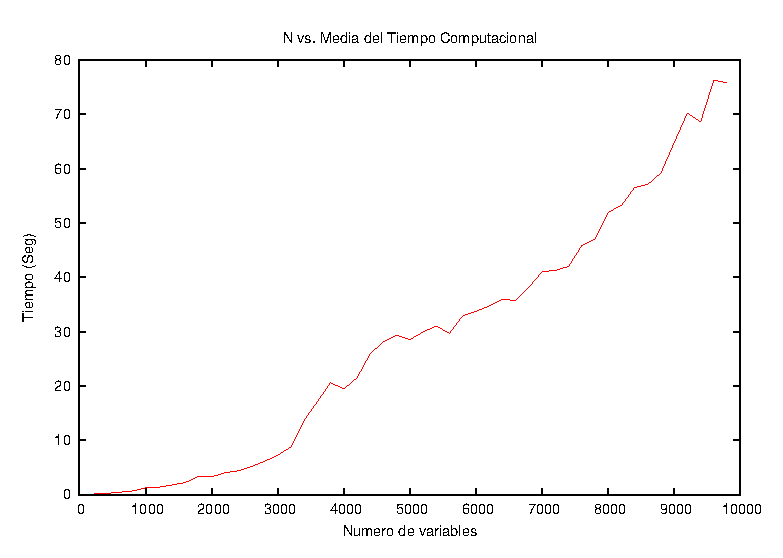
\includegraphics[scale=0.6]{img/Media_Tiempo_1.eps}
%\caption{}
%\end{figure}
%
%\begin{figure}[h]
%\center
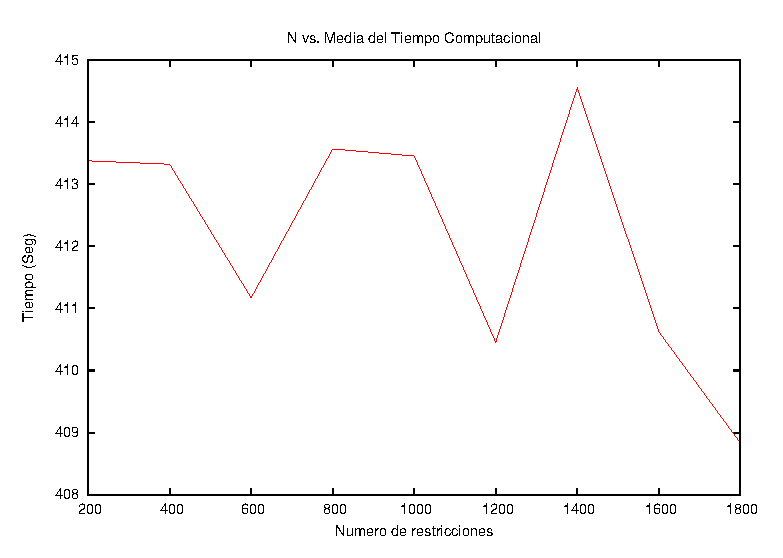
\includegraphics[scale=0.6]{img/Media_Tiempo_2.eps}
\caption{En la izquierda la media contra tiempo con $n=200*i$ e $i \in \{1,2,..,50 \}$ donde $m=n/2$ y en la deracha la media contra tiempo con $n=2000$ donde $m=200*i$.}
\label{img:Media}
\end{figure*}

\begin{figure*}[h]
\center
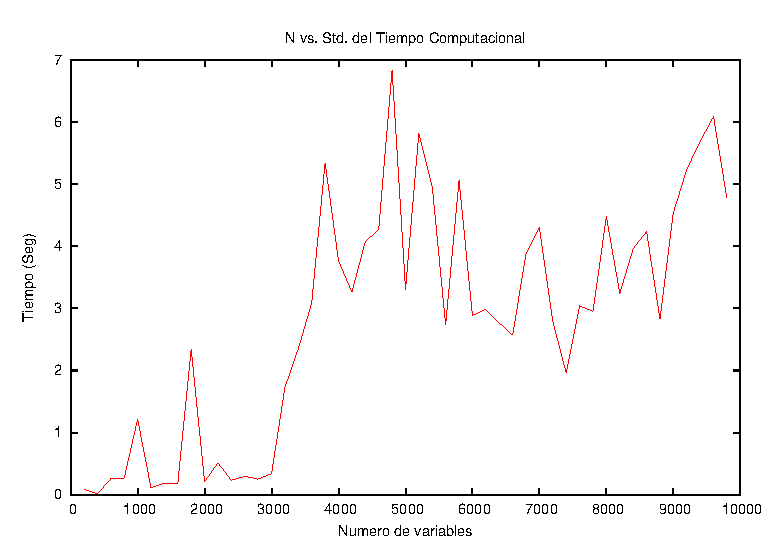
\includegraphics[scale=0.6]{img/Varianza_Tiempo_1.eps}
%\caption{Varianza contra tiempo con $n=200*i$ e $i \in \{1,2,..,50 \}$ donde $m=n/2$.}
%\end{figure}
%
%\begin{figure}[h]
%\center
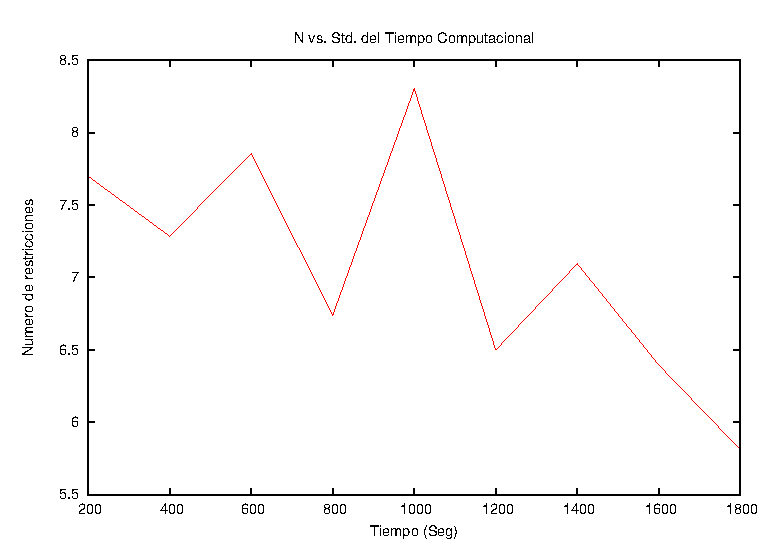
\includegraphics[scale=0.6]{img/Varianza_Tiempo_2.eps}
\caption{En la izquierda la varianza contra tiempo con $n=200*i$ e $i \in \{1,2,..,50 \}$ donde $m=n/2$ y en la derecha la varianza contra tiempo con $n=2000$ donde $m=200*i$.}
\end{figure*}

\subsection{Problema de asignación de ambulancias aéreas}
El objetivo es determinar una signación de costo mínimo de helicoperos a los sitios que satisfacen la demanda proyectada para el siguiente periodo de tiempo.
%
\subsubsection{Declaración del problema}
El servicio de ambulancia tiene un conjunto de ubicaciones con un número de helicópteros en cada sitio.
%
Cada sitio requerido es visitado por su respectivo helicoptero.
%
Existe un costo en la reasignación de un helicóptero a un sitio distinto.
%
Por lo tanto, el servicio proporcionado desea determinar un costo de asignación mínimo de helicópteros a los sitios para satisfacer la demanda en el siguiente periodo de asignación proyectado en cada sitio.
%
\subsection{Formulación matemática}
Dado un conjunto de ubicaciones, las distancias entre las ubicaciones, el número de helicópteros recientemente asignados a cada ubicación, la demanda proyectada para cada ubicación y el costo por ilómetro,
%
El objetivo del problema de asignación de ambulancias es determinar el costo mínimo en la reasignación para satisfacer la demanda proyectada.
%
El problema puede ser formulado como un problema de programación lineal porque la función objetivo y las restricciones son todas funciones lineales.
%
Los pares de distancia son calculadas con la distancia Euclídea.
%


\subsubsection*{Asignar}
\textbf{L} = el conjunto de ubicaciones.


\subsubsection*{Parámetros}
\begin{itemize}
\item \textbf{$x_i$} = la coorenada X para la ubicación de $i, \forall i \in L$.
\item \textbf{$y_i$} = la coorenada Y para la ubicación de $i, \forall i \in L$.
\item \textbf{$d_i$} = demanda proyectada para el sigueinte periodo de la ubicación $i, \forall i \in L$.
\item \textbf{$s_i$} = número de helicópteros recientemente asignados a la ubicación $i, \forall i \in L$.
\item \textbf{$c$} = costo de transportar por kilómetro.
\item \textbf{$dist_{ij}$} = Distancia Euclídea entre la ubicación $i$ y la ubicación $j$ $, \forall i \in L, \forall j \in L$.
\item \textbf{$dist_{ij}$} = $\sqrt{ (x_j - x_i)^2 + (y_j - y_i)^2 }$.
\end{itemize}

\subsubsection*{Variables}
$z_{ij}$ = número de helicópteros a ser desplazados de la ubicación $i$ a la $j$, $\forall i \in L, \forall j \in L$.

\subsubsection*{Función objetivo}
\begin{equation}
Minimizar \quad \sum_{(i,k) \in LxL} dist_{ij} * c * z_{ij}
\end{equation}
\subsubsection*{Restricciones}
Restricciones de balance para cada ubicación $i$ en el conjunto $L$.
\begin{equation}
\sum_{j \in L} z_{ij} + s_i = d_i 6 \sum_{j \in L} z_{ij}, \forall i \in L
\end{equation}

Como ejemplo, se considera un servicio de ambulancias aéreas con 5 ubicaciones en Midwest.
%
La empresa tiene la necesidad de reubicar a los helicópteros basados en le demanda mensual proyectada para cada ubicación.
%
El costo de reasignar un helicóptero del sitio $i$ al sitio $j$ es de $100$ pesos por kilómetro.
%
Se muestra la tabla de cada ubicación.
\begin{table}[]
\centering
\caption{Información de los helicópteros asignados}
\label{my-label}
\begin{tabular}{c|c|c|c|c}
\hline
\textbf{} & \textbf{X - Coord} & \textbf{Y-Coord} & \textbf{\# Assigned} & \textbf{Projected Demand} \\ \hline
Location \#1 & 36 & 20 & 6 & 7 \\ \hline
Location \#2 & 23 & 30 & 2 & 3 \\ \hline
Location \#3 & 23 & 56 & 3 & 2 \\ \hline
Location \#4 & 10 & 15 & 3 & 4 \\ \hline
Location \#5 & 5 & 5 & 4 & 2 \\ \hline
\end{tabular}
\end{table}

La solución al problema es: $z_{3,2}=1$, $z_{5,1}=1$, y $z_{5,4}=1$ con un valor de la función objetivo de $7161.87$.
%
La distancia están como sigue: $dist_{3,2}=26$, $dist_{5,1}=34.438$, y $dist_{5,4}=11.180$.

